\documentclass[fontsize=10pt,paper=b5,open=any,
twoside=no,toc=listof,toc=bibliography,headings=optiontohead,
captions=nooneline,captions=tableabove,english,DIV=15,numbers=noenddot,final,parskip=half-,
headinclude=true,footinclude=false,BCOR=0mm]{scrartcl}
\pdfvariable suppressoptionalinfo 512\relax
\synctex=1

\author{Valentin Boettcher}
\usepackage{hirostyle}
\usepackage{hiromacros}
\addbibresource{references.bib}

\title{The non-Markovian Quantum Walk for Finite Baths (Summary)}
\date{2023}
\graphicspath{{plots}}


\begin{document}
\maketitle
\tableofcontents
\newpage
Herein we report how to reproduce the behavior found for non-Markovian
quantum walk in the continuum limit with the Born approximation
presented in \refcite{Ricottone2020} using a finite number of
reservoir states and a finite coupling strength. The final result is
presented in \cref{fig:example_finite_vs_continuum}. We introduce the
details of the model in \cref{sec:model-relev-observ} and explain how
\cref{fig:example_finite_vs_continuum} was produced in
\cref{sec:finite-size-efects}.
\begin{figure}[H]
  \centering
  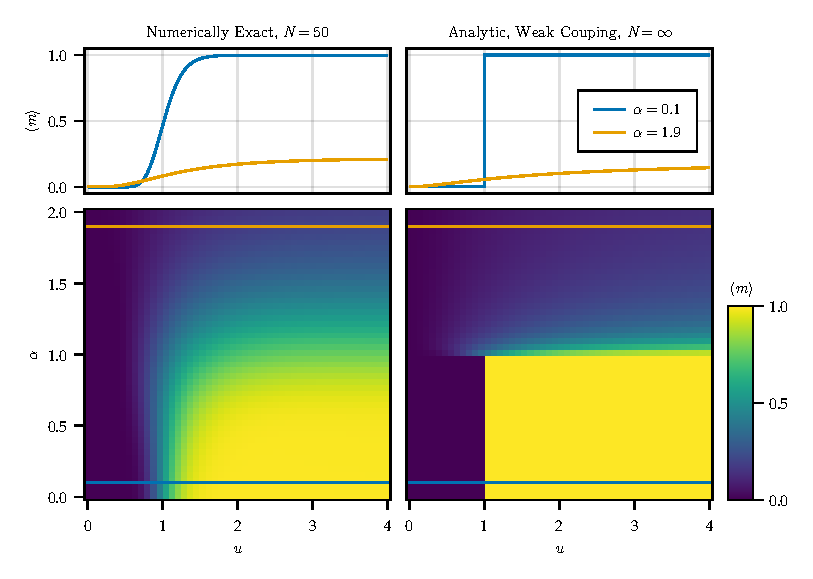
\includegraphics{plots/example_finite_vs_continuum}
  \caption{\label{fig:example_finite_vs_continuum} The full phase
    diagram and constant-\(α\) cuts obtained through numerical
    diagonalization and though an analytic estimate in the weak
    coupling limit for \(g_{0}=0.2 ω_{c}\).}
\end{figure}

\section{Model and relevant Observables}
\label{sec:model-relev-observ}

The basic model is given by~\cite{Ricottone2020}
\begin{align}
  \label{eq:58}
  H &= H_{A} +H_{\bar{A}} + V\\
  H_{A} &= ∑_{m=0}^{L-1}ε_{A} a_{A,m}^{†}a_{A,m} \\
  H_{\bar{A}} &= ∑_{m=0}^{L-1}{(ε_{A} + ω)a_{B,m}^{†}a_{B,m}}+
                   ∑_{j}\bqty{ε_{j} b_{j,m}^{†}b_{j,m} + g_{j}
                   \pqty{a_{B,m}^{†}b_{j,m} + \hc}}\\
  V&=∑_{m=0}^{L-1} v\pqty{a_{A,m}^{†}a_{B,m}+ u a_{A,m}^{†}a_{B,m+1}} + \hc,
\end{align}
which describes an SSH chain with \(L\) sites, periodic boundary
conditions, site energy detuning \(ω\) and extra ``reservoir'' modes
\(b_{j,m}\) in each unit cell that are coupled to the \(B\) sites. We
are using second quantized notation here, where
\(a^{†}_{X,m}\ket{0} = \ket{X,m}\) creates a particle at sublattice
site \(X\) and lattice site \(m\) and
\(b^{†}_{j,m}\ket{0} = \ket{j,m}\) creates a particle in the \(j\)th
reservoir mode at site \(m\). The \(a\) and \(b\) operators obey the
usual bosonic commutation relations. This is equivalent to the single
particle picture in \refcite{Ricottone2020}, as this Hamiltonian
preserves excitations.

We are interested in the evolution of an initial state of a particle,
the ``walker'', \(\ket{\psi(0)}=\ket{A,0}\) with respect to the
parameter \(u\) and the structure of the reservoir, namely the choice
of \(ε_{j}\) and \(g_{j}\). An observable that is sensitive to the
bath structure \emph{and} the topological phase of the SSH bare
model\footnote{This is understood as setting \(g_{j}=0\) and \(ω=0\)
  leaving \(v\) and \(u\) unchanged.} is the mean displacement
\begin{equation}
  \label{eq:59}
  \ev{m(t)} \equiv ∑_{m}m {ρ_{\bar{A},m}(t)}
\end{equation}
where
\(ρ_{\bar{A},m}(t) = {∑_{l\neq A} \abs{\braket{l,m}{ψ(t)}}^{2}}\) is
the probability that the walker does reside in cell \(m\) but not the \(A\) site in
cell \(m\) at time \(t\).

To simplify calculations, we exploit the translational symmetry of the
model to express it in momentum space and remove the \(B\) sites by a
Schrieffer-Wolff transformation for large \(ω\) resulting in
\(H=∑_{k}H(k)\) with
\begin{equation}
  \label{eq:61}
  H(k) = {ω}_{A} a_{k,A}^{†}a_{k,A}+ ∑_{j} \bqty{{ω}_{j} b_{j,m}^{†}b_{j,m}
    + \pqty{\frac{v(k)}{\abs{v(0)}}η_{j} a_{k,A}^{†}b_{j,m}+ \hc}},
\end{equation}
where \(k=\frac{2π n}{L}\) for \(n\in[0, L-1]\), \(L\in\NN\),
\(c_{k,l} = \frac{1}{L}\) and
\begin{equation}
  \label{eq:72}
  v(k)=v+v\prime\eu^{\iu k}=v(1+u)\eu^{\iu k} = \abs{v(k)}\eu^{\iu ϕ(k)}.
\end{equation}


The mean displacement can be re-expressed in terms of momentum space quantities
\begin{equation}
  \label{eq:62}
  \begin{aligned}[t]
  \ev{m(t)} &= ∑_{k} \pqty{\frac{1}{L}-ρ_{A}\pqty{k,
              t}}\pdv{ϕ}{k}\pqty{k}
  \end{aligned}
\end{equation}
where \(ρ_{A}(k,t)=\abs{\braket{A,k}{ψ(t)}}^{2}\) with
\(\ket{ψ(0)}=\ket{A,k=0}=a^{†}_{A,k=0}\ket{0}\).

As \(\ev{m(t)}\) can exhibit persistent oscillations in general as can
be seen in the \(α=1.9\) case in \cref{fig:mean_displacement_example},
we instead consider a time average
\begin{equation}
  \label{eq:69}
  \ev{m} \equiv \frac{1}{τ_{h} - τ_{l}} ∫_{τ_{l}}^{τ_{h}}\ev{m(t)} \dd{t},
\end{equation}
with \(τ_{l}\) and \(τ_{h}\) chosen appropriately to avoid transient
effects and Poincaré recurrence due the possibly finite size of the
reservoir. This means, that the state of the system comes arbitrary
close to its initial state in finite time. As we are interested in
reproducing the behavior of the infinite system, we have to work on
time-scales where this effect doesn't come to play.

In the continuum limit we can ignore transient effects and choose
\(τ_{l}=0\) and take the limit of \(τ_{h}\to ∞\) obtaining
\begin{equation}
  \label{eq:60}
  \ev{m} =  \lim_{T\to ∞} \frac{1}{T} ∫_{0}^{T}\ev{m(t)}\dd{t}.
\end{equation}

If \(ρ_{A}(k,t)\xrightarrow{t\to ∞}0\) for all \(k\), the long-time
averaged mean displacement \(\ev{m}\) exhibits a universal behavior
corresponding to the topological phase of the original SSH chain
\begin{equation}
  \label{eq:63}
  \ev{m} = θ(u-1),
\end{equation}
as in the right panel of \cref{fig:example_finite_vs_continuum} for
\(α<1\).

The structure of the reservoir is described by the
spectral density which we choose to take the form of a power law
\begin{equation}
  \label{eq:64}
  J(ω)
  =
  \begin{cases}
    \pqty{g_{0}^{2}\frac{(α+1)}{ω_{c}^{α+1}}} ω^{α} & \mathrm{for}\; 0\leq
                                               ω\leq ω_{c}\\
    0 & \mathrm{otherwise},
  \end{cases}
\end{equation}
where \(ω_{c}\) is called the cutoff frequency and \(α\) controls how
fast \(J(ω)\) approaches zero for \(ω\to 0\). The coupling strength
\(g_{0}\) can be expressed by the couplings through
\begin{equation}
  \label{eq:70}
  g_{0} = \sqrt{∑_{j}\abs{η_{j}}^{2}}.
\end{equation}
For finite-size reservoirs, a simple choice for the \(ω_{j}\) and
\(η_{j}\) is
\begin{equation}
  \label{eq:65}
  \begin{aligned}
    Δω &= \frac{ω_{c}}{N} & ω_{j} &= Δω \pqty{j + \frac{1}{2}} & η_{j}^{2}
    &= J(ω_{j}) Δω,
  \end{aligned}
\end{equation}
which recovers the behavior of \cref{eq:64} in the limit \(N\to ∞\).

It was shown in \refcite{Ricottone2020} using the Born approximation
and taking the continuum limit for the reservoir and \(L=∞\), that
\(\ev{m}\) matches \cref{eq:63} precisely for \(α<1\) whereas it takes
on non-universal values for \(α>1\). This behavior can also be
obtained without employing the Born approximation and is presented in
the right column of \cref{fig:example_finite_vs_continuum}.


\section{Effects of Finite Coupling and Finite
  Reservoir Size}
\label{sec:finite-size-efects}

The finite size of the reservoir will in general wash out the sharp
phase transitions observed in \refcite{Ricottone2020}. Additionally it
will lead to recurrences in the dynamics around the time
\begin{equation}
  \label{eq:71}
  τ_{R}=\frac{2π}{Δω}
\end{equation}
where \(N\) is the number of reservoir modes. On the other hand
\(ρ_{A}(k,t)\) decays with a rate \(Γ \sim π g_{0}^{2} / ω_{c}\). It
is therefore necessary to have \(1/Γ \ll τ_{R}\), which gives a lower
bound for the number of reservoir states required at a certain
coupling strength
\begin{equation}
  \label{eq:73}
  \frac{ω_{c}^{2}}{2π^{2}g_{0}^{2}} \ll N.
\end{equation}

To limit the number of reservoir states required, we would like to
choose a finite \(g_{0}\).  In this case level repulsion shifts the
effective energy of the \(A\) site.  This Lamb shift can be countered
by choosing a specific value of the \(A\) site energy
\begin{equation}
  \label{eq:66}
  ω_{A} = ∑_{j}\frac{\abs{η_{j}}^{2}}{ω_{j}} = \frac{1}{N} ∑_{j}
  J(ω_{j}) \frac{ω_{c}}{ω_{j}},
\end{equation}
where \(ω_{A}\) is independent of \(u\) but still depends on \(α\).

With these considerations in mind we do choose the parameters of the
model and study the behavior of \(\ev{m}\) for a specific \(u\) and
\(α\) in \cref{fig:mean_displacement_example}.

For the concrete parameter choice in
\cref{fig:mean_displacement_example,fig:example_finite_vs_continuum}
we find, that \(\ev{m(t)}\) approaches the universal value of
\(\ev{m}=1\) very close and that the decay and revival time scales are
well separated. Therefore, the time average of \(\ev{m(t)}\) in
\cref{eq:69} can be taken over an interval of
\(\bqty{τ_{l}, τ_{h}}=\bqty{0.5 τ_{R}, 0.95 τ_{R}}\), where other
choices would also be valid.  The lower end of the time interval is
chosen to avoid transient behavior, whereas the upper end is chosen to
stay well clear of the revivals.
\begin{figure}[H]
  \centering
  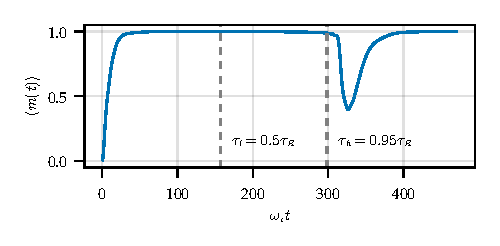
\includegraphics[width=.8\linewidth]{plots/mean_displacement_example_simple}
  \caption{\label{fig:mean_displacement_example} The mean \(\ev{m}\)
    displacement over time for two values of \(α\), \(u=4\), \(N=50\)
    in relation to the recurrence time \(τ_{R}\). The mean
    displacement for \(α=1.9\) exhibits persistent oscillations for
    \(α=1.9\) and doesn't converge to its steady state value which is
    an artifact of the finite recurrence time and the \(k\) dependence
    of \(ρ_{A}(k,t)\) for finite \(u<∞\) at finite coupling
    strengths.}
\end{figure}

We are now in a position to discuss the full phase diagram for the
finite system in \cref{fig:example_finite_vs_continuum}. Despite the
finite size effects, the resemblance to the continuum/weak-coupling
limit is clearly visible when comparing the two sides of
\cref{fig:example_finite_vs_continuum}.  The coupling strength
\(g_{0}=0.2 ω_{c}\) leads to a saturation of the mean displacement
\(\ev{m}\to 1\) for \(u>2\), \(α\lesssim 1\) and \(N=50\) while the
behavior of the model is still far away from the ultra-strong coupling
limit, where \(\ev{m(t)}\sim \cos[2](Ω t)\) for some \(Ω\) and thus
\(\ev{m}=1/2 \) for all choices of \(u,\, α\).

\printbibliography{}
\end{document}


%%% Local Variables:
%%% mode: latex
%%% TeX-master: t
%%% TeX-output-dir: "output"
%%% TeX-engine: luatex
%%% End:
